\documentclass{beamer}
\usepackage[latin1]{inputenc}

\usetheme{Madrid}
\usecolortheme{default}
\usepackage{amsmath}
\usepackage{amssymb,amsfonts,amsthm}
\usepackage{txfonts}
\usepackage{tkz-euclide}
\usepackage{listings}
\usepackage{adjustbox}
\usepackage{array}
\usepackage{tabularx}
\usepackage{gvv}
\usepackage{lmodern}
\usepackage{circuitikz}
\usepackage{tikz}
\usepackage{graphicx}
\usepackage{gensymb}
\usepackage{physics}

\setbeamertemplate{page number in head/foot}[totalframenumber]

\usepackage{tcolorbox}
\tcbuselibrary{minted,breakable,xparse,skins}



\definecolor{bg}{gray}{0.95}
\DeclareTCBListing{mintedbox}{O{}m!O{}}{%
  breakable=true,
  listing engine=minted,
  listing only,
  minted language=#2,
  minted style=default,
  minted options={%
    linenos,
    gobble=0,
    breaklines=true,
    breakafter=,,
    fontsize=\small,
    numbersep=8pt,
    #1},
  boxsep=0pt,
  left skip=0pt,
  right skip=0pt,
  left=25pt,
  right=0pt,
  top=3pt,
  bottom=3pt,
  arc=5pt,
  leftrule=0pt,
  rightrule=0pt,
  bottomrule=2pt,
  toprule=2pt,
  colback=bg,
  colframe=orange!70,
  enhanced,
  overlay={%
    \begin{tcbclipinterior}
    \fill[orange!20!white] (frame.south west) rectangle ([xshift=20pt]frame.north west);
    \end{tcbclipinterior}},
  #3,
}
\lstset{
    language=C,
    basicstyle=\ttfamily\small,
    keywordstyle=\color{blue},
    stringstyle=\color{orange},
    commentstyle=\color{green!60!black},
    numbers=left,
    numberstyle=\tiny\color{gray},
    breaklines=true,
    showstringspaces=false,
}
\title{5.2.28}
\date{19th september, 2025}
\author{Vishwambhar - EE25BTECH11025}

\begin{document}

\frame{\titlepage}
\begin{frame}{Question}
Solve the system of linear equations:
\begin{align}
    5x-8y=-1\\
    3x-\frac{24}{5}y=\frac{-3}{5}
\end{align}
\end{frame}

\begin{frame}{Given}
Given
\begin{align}
    \myvec{5&-8}\vec{x}=-1;\myvec{3&\brak{\frac{-24}{5}}}\vec{x}=\frac{-3}{5}\\
    A=\myvec{5&-8\\3&\brak{\frac{-24}{5}}};
    \vec{x}=\myvec{x\\y};
    \vec{b}=\myvec{-1\\ \brak{\frac{-3}{5}}}\\
    A\vec{x}=\vec{b}
\end{align}
\end{frame}

\begin{frame}{Given}
Let:\\
Rank of coefficient matrix $=r$\\
Rank of Augmented matrix $=r_a$\\
Order of coefficient matrix $=n$\\
\end{frame}

\begin{frame}{Solving}
Augmented Matrix:
\begin{align}
    \augvec{2}{1}{5&-8&-1\\3&\brak{\frac{-24}{5}}&\brak{\frac{-3}{5}}}\\R_2 \rightarrow R_2-\frac{3}{5}R_1\\
    \augvec{2}{1}{5&-8&-1\\0&0&0}\\
    r=1;r_a=1;n=2\\
    \because r=r_a<n
\end{align}
Infinite solutions exist for the given system of linear equations.
\end{frame}

\begin{frame}[fragile]
    \frametitle{C Code}
    \begin{lstlisting}
#include<stdio.h>

void make_data(double *points){
    double n = 2;
    points[0] = 5;
    points[1] = -8;
    points[2] = -1;
    points[3] = 3;
    points[4] = -4.8;
    points[5] = -0.6;
    points[6] = 2;
}
    \end{lstlisting}
\end{frame}

\begin{frame}[fragile]
    \frametitle{C Code}
    \begin{lstlisting}
void processing(double rA, double rB, double n, double X, double Y){
    if(rA==rB&&rB==n){
        printf("Unique solution exists for the given system of linear equations.\n");
        printf("The solution for the given system of linear equations is: x=%.2lf, y=%.2lf", X, Y);
    }
    else if(rA==rB&&rA!=n){
        printf("Infinite solutions exist for the given system of linear equations in 2 variables.");
    }
    else{
        printf("No solution exists for the given system of linear equations in 2 variables");
    }
}
    \end{lstlisting}
\end{frame}


\begin{frame}[fragile]
    \frametitle{Python Code 1}
    \begin{lstlisting}
import ctypes as ct
import sympy as sp

lib = ct.CDLL("./problem.so")
entry = ct.c_double*7
lib.make_data.argtypes = [ct.POINTER(ct.c_double)]
lib.processing.argtypes = [ct.c_double, ct.c_double, ct.c_double, ct.c_double, ct.c_double]
data = entry()
lib.make_data(data)
A = sp.Matrix([[data[0], data[1], data[2]],
                   [data[3], data[4], data[5]]])
B = sp.Matrix([[data[0], data[1]],
                   [data[3], data[4]]])
    \end{lstlisting}
\end{frame}

\begin{frame}[fragile]
    \frametitle{Python Code 1}
    \begin{lstlisting}
C = ([data[0], data[3]])
D = ([data[1], data[4]])
E = data[2]
F = data[5]
n = data[6]
def get_data():
    return C, D, E, F
rA = A.rank()
rB = B.rank()
rref_matrix, pivots = A.rref()
lib.processing(rA, rB, n, rref_matrix[0,2], rref_matrix[1,2])
    \end{lstlisting}
\end{frame}

\begin{frame}[fragile]
    \frametitle{Python Code 2}
    \begin{lstlisting}
import matplotlib.pyplot as plt
import numpy as np
from call import get_data

C, D, E, F = get_data()

x = np.linspace(-10, 10, 100)
y = -((C[0]*x)-E)/D[0]

X = np.linspace(-15, 15, 100)
Y = -((C[0]*X)-E)/D[0]
    \end{lstlisting}
\end{frame}

\begin{frame}[fragile]
    \frametitle{Python Code 2}
    \begin{lstlisting}
plt.plot(X, Y, '-k')
plt.plot(x, y, '-r')
plt.text(-13.64, -8.96, r'$5x-8y=-1$', fontsize=10, color='black')
plt.text(1.06, 1.08, r'$3x-\frac{24}{5}y=-\frac{3}{5}$', fontsize=10, color='black')
plt.xlabel('X-axis')
plt.ylabel('Y-axis')
plt.axis('equal')
plt.grid(True)
plt.savefig("../figs/plot.png")
plt.show()   \end{lstlisting}
\end{frame}

\begin{frame}{Plot}
    \begin{figure}
        \centering
        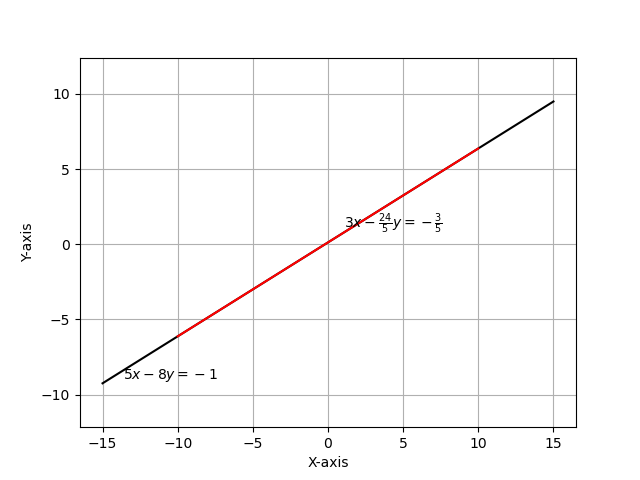
\includegraphics[width=0.5\columnwidth]{../figs/plot.png}
        \caption{Plot of the given line equations}
        \label{fig:fig}
    \end{figure}
\end{frame}
\end{document}
